\documentclass[aps,prb,reprint,superscriptaddress, a4paper]{revtex4-1}
%\documentclass[aps,prl,preprint,superscriptaddress]{revtex4-1}
%\documentclass[aps,prl,reprint,groupedaddress]{revtex4-1}

% You should use BibTeX and apsrev.bst for references
% Choosing a journal automatically selects the correct APS
% BibTeX style file (bst file), so only uncomment the line
% below if necessary.
%\bibliographystyle{apsrev4-1}
\usepackage{siunitx}
\usepackage[shell]{gnuplottex}
%\usepackage[miktex]{gnuplottex}
\usepackage{float}
\usepackage{hyperref}
\usepackage{pgf}
\usepackage{graphicx}
\usepackage{amsmath}
\usepackage{tikz}
\usepackage{bm}
\usepackage{structuralanalysis}
\usepackage{color}
\usepackage{diagbox}
\usepackage[utf8]{inputenc} % input encoding

\usepackage{enumitem}
\setlist[description]{leftmargin=1pt,labelindent=1pt,itemsep=-2pt,topsep=1pt}
\renewcommand{\descriptionlabel}[1]{
            \hspace\labelsep \upshape #1
                                    }
\definecolor{SERorange}{HTML}{FFA500}
\definecolor{SERred}{HTML}{F00000}
\definecolor{SERgray}{HTML}{909090}
\definecolor{SERwhite}{HTML}{F8F8F8}

\definecolor{SERgreen}{HTML}{34B853}
\definecolor{SERorange2}{HTML}{F64724}
\definecolor{SERyellow}{HTML}{FFCC00}
\definecolor{SERblue}{HTML}{4295F9}




%\usepackage{enumitem}
\begin{document}

% Use the \preprint command to place your local institutional report
% number in the upper righthand corner of the title page in preprint mode.
% Multiple \preprint commands are allowed.
% Use the 'preprintnumbers' class option to override journal defaults
% to display numbers if necessary
%\preprint{}

%Title of paper
\title{}

% repeat the \author .. \affiliation  etc. as needed
% \email, \thanks, \homepage, \altaffiliation all apply to the current
% author. Explanatory text should go in the []'s, actual e-mail
% address or url should go in the {}'s for \email and \homepage.
% Please use the appropriate macro foreach each type of information

% \affiliation command applies to all authors since the last
% \affiliation command. The \affiliation command should follow the
% other information
% \affiliation can be followed by \email, \homepage, \thanks as well.
\author{Sebasti\'{a}n Echeverri Restrepo}
\email[]{sebastian.echeverri.restrepo@skf.com}
\affiliation{SKF Engineering \& Research Centre (ERC), SKF B.V., Nieuwegein, The Netherlands}
\affiliation{Department of Physics, King's College London, Strand, London WC2R 2LS, United Kingdom}
\author{James P. Ewen}
\affiliation{Department of Mechanical Engineering, Imperial College London, London SW7 2AZ, England, UK}
\author{Daniele Dini}
\affiliation{Department of Mechanical Engineering, Imperial College London, London SW7 2AZ, England, UK}

%Collaboration name if desired (requires use of superscriptaddress
%option in \documentclass). \noaffiliation is required (may also be
%used with the \author command).
%\collaboration can be followed by \email, \homepage, \thanks as well.
%\collaboration{}
%\noaffiliation

\date{\today}

\begin{abstract}


\end{abstract}

% insert suggested PACS numbers in braces on next line
\pacs{}


%\maketitle must follow title, authors, abstract, \pacs, and \keywords
\maketitle



% body of paper here - Use proper section commands
% References should be done using the \cite, \ref, and \label commands
%%%%%%%%%%%%%%%%%%%%%%%%%%%%%%%%%%%%%%%%%%%%%%%%%
%%%%%%%%%%%%%%%%%%%%%%%%%%%%%%%%%%%%%%%%%%%%%%%%%
%%%%%%%%%%%%%%%%%%%%%%%%%%%%%%%%%%%%%%%%%%%%%%%%%

\section{Introduction}


Lubrication is one of the most important factors  that determine the performance and useful life of roller bearings. Lubricants are used to minimise friction and prevent excessive wear between  adjacent parts sliding or rolling against each other. Lubricants work by generating a thin film that separate the surfaces in contact. Additionally, the lubricant should also serve as a mean to dissipate the heat generated by friction, and  it should help prevent corrosion and the ingress of moisture and contaminants to the contact surface. 

Lubricants for industrial applications are normally produced as a mixture of  a base oil and   additive packages.  Base oils  are divided into five general categories based on the refining method and the base oil's properties, as stated by the American Petroleum Institute (API)\cite{API}.

Paraffinic base oils,  sometimes referred to as  Group I or II, are usually characterised by high viscosity indices and flash points, and  resistance to oxidation. They  are produced using solvent-extraction,  solvent-refining, or hydrogenation, with the aim of creating an oil with  a marginal content of undesirable components such as ring structures and aromatics. This means that paraffinic oils are mainly  composed of straight-chain or branched aliphatic hydrocarbons, that is,  alkanes (parafins) and their isomers.


Alkanes are acyclic saturated hydrocarbons described by the general chemical formula $\text{C}_{n}\text{H}_{2n+2}$. In simpler terms, they are chains of carbon and hydrogen atoms in which all the carbon-carbon bonds are single. The simplest alkane $\left(n=1\right)$ is methane, and they can grow in complexity to arbitrarily long chains. Usually, higher alkanes (composed of 16 carbon atoms or more) are  main components of lubricating oil.


According to the \textit{Encyclopedia of Tribology}\cite{Wang2013a}, Thin Film Lubrication (TFL) is a lubrication state with the lubricant film from a few nanometers to tens of nanometers, which is a lubrication regime between boundary lubrication and elastohydrodynamic lubrication (EHL). At the length scales of TFL and for dealing with simple molecules, like the linear alkanes that compose paraffinic base oils, Molecular Dynamics (MD) comes as an ideal tool for the detailed study of the tribological phenomena resulting from  the relative movement of two surfaces separated by a lubricant film. In the latest years, thanks to the constant increase in available computational power and the development of more accurate force fields, it has become possible to routinely perform larger and longer MD simulations of TFL. We are now able to get insights about the behaviour of lubricants with a detail that goes down to the scale of single atoms. 

One of the topics that has been studied using MD is  the effect of pressure on TFL. In reference \cite{Thompson1992}, a MD study of highly confined chain molecules  detected  changes in the diffusion constant and the response to shear caused by the formation of a crystalline or glassy phase across the film at high pressures. Similarly, in \cite{Robbins1996} the difference in behaviour between of molecularly-thin and macroscopic lubricant films is discussed; they concluded that the differences between molecular and macroscopic scale friction is related to phase transformations induced by confinement.   

Phase transitions of boundary-driven sheared Lennard-Jones (LJ) liquids have also been studied using MD. These studies showed that the fluids will show different  but well defined phases depending on the external constraints (velocity and pressure), a behaviour that can be well described by a phase diagram \cite{Heyes2012}. It was also found that single component LJ liquids form semicrystalline arrangements and behave more like traction fluids, while binary mixtures discourages crystallization and give a more classical tribological response, closer to that of lubricants \cite{Gattinoni2013}. Another study found that, due to the nonequilibrium phase adopted by fluid, the friction coefficient does not necessarily echo the classical friction relations between macroscopic bodies \cite{Mackowiak2016}.


MD simulations of TFL have also been used to study confined linear polymers. For this type of systems, in general,  simulations show that in the narrow interface between  the polymer melt and the surface,  the properties  of the polymer melt deviate significantly from their  bulk values and present a pronounced spatial dependence\cite{Bitsanis1990}; for instance, the viscosity  is much higher than in the middle of the film and most of the shear thinning takes place in the absorbed layer \cite{Manias1996}. In \cite{Sivebaek2010} it was found that, in the case of a polymer melt sliding against a hard substrate, the  frictional shear stress increases monotonically with the sliding velocity. In similar simulations by the same author\cite{Sivebaek2012}, it was also found that the logarithm of the effective viscosity depends linearly on the logarithm of the shear rate. 

Slip between lubricant and moving surfaces is another topic for which the atomic scale resolution of MD is specially well suited. In   \cite{MARTINI2008} two different molecular mechanisms by which slip occur were presented.  In the first form, slip is a rate process between equilibrium sites: following Arrhenius dynamics, atoms hop between valleys along the solid surface from one equilibrium site to another. The second form, consist on the relative movement of the entire liquid layer with respect to the surface  and  is observed at high enough forcing. In a similar work, the same author\cite{Martini2008a},  showed that as shear rate increases, the amount of slip approaches  a constant value.



In the present work xxxxxx



%%%%%%%%%%%%%%%%%%%%%%%%%%%%%%%%%%%%%%%%%%%%%%%%%
%%%%%%%%%%%%%%%%%%%%%%%%%%%%%%%%%%%%%%%%%%%%%%%%%
%%%%%%%%%%%%%%%%%%%%%%%%%%%%%%%%%%%%%%%%%%%%%%%%%
\section{Methods}

\subsubsection{Simulation Details}

The generation of all the initial configurations is done using the software LAMMPS\_builder\footnote{\url{https://github.com/JE1314/LAMMPS_builder}} \cite{Ewen2017b,Jewett2013,HjorthLarsen2017}. The systems consist of two parallel flat surfaces separated by a region containing a lubricant, see Figure \ref{fig:Steps}. Periodic boundary conditions were applied in the x and y directions.

The lubricant is generated as a polymer melt of alkanes. Three different types of alkanes are used, the only difference between them being the number of carbons in the backbone:  hexadecane (C16),  triacontane (C30) and  hexacontane (C60). For all the cases, a  total number of 19200 carbon atoms    are inserted into the system; this corresponds to 1200, 640 and 320 chains for C16, C30 and C60, respectively.

The surfaces are composed of $\text{Fe}$ and $\text{O}$ atoms arranged in a hexagonal structure to form hematite $\left(\text{Fe}_2\text{O}_3\right)$. The initial lattice parameters for the $\text{Fe}_2\text{O}_3$ unit cell are $a=b=\SI{5.029}{\angstrom}$ and  $c=\SI{13.730}{\angstrom}$ with the angles $\alpha=\beta=\SI{90}{\degree}$ and  $\gamma=\SI{120}{\degree}$. The surfaces are oriented in such a way that   $\left[001\right]$ direction points towards z (perpendicular to the surface) and  $\left[100\right]$ towards x (shearing direction). For all the simulations, the thickness of the surfaces is equivalent to one lattice constant, $c=\SI{13.730}{\angstrom}$; the size of the surface in the  y and x direction are $16a=\SI{80.464}{\angstrom}$ and $16a\sin{\SI{60}{\degree}}=\SI{78.394}{\angstrom}$. The dimensions are selected to be large enough to prevent self interaction of individual alkane chains.


Classical MD simulations were performed using the software LAMMPS \cite{Plimpton1995}. The velocity-Verlet algorithm was used to integrate the equations of motion using a  time-step of \SI{1.0}{\femto\second}. Fast-moving bonds involving hydrogen atoms were constrained with the SHAKE algorithm \cite{Ryckaert1977}. The interaction between the atoms in the alkane chains are defined by the all atom L-OPLS force-field \cite{Jorgensen1988,Siu2012}, as recommended in \cite{Ewen2016a} for this type of simulations. To define the behaviour of the atoms in the surfaces, the approach taken in \cite{Savio2012} is followed.  Cross-interactions between atoms in the surfaces and in the lubricant were evaluated using  geometric mean mixing rules \cite{Jorgensen1996}. Electrostatic interactions were evaluated using a slab implementation of the particle-particle-particle-mesh (PPPM) algorithm \cite{Yeh1999} with a relative accuracy in the forces of \SI{1e-7}{}. 




\begin{figure*}
    	\begin{center}
		
		\begin{tikzpicture}
			\node[anchor=south west,inner sep=0] (fig_axes) at (0,0){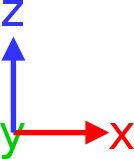
\includegraphics[width=0.04\textwidth]{Data/Images/Axes.png}};
			%%%%%
			\node[anchor=south west,inner sep=0] (fig_Steps0) at ({(\textwidth-\textwidth/10)*0.00+\textwidth/20},0){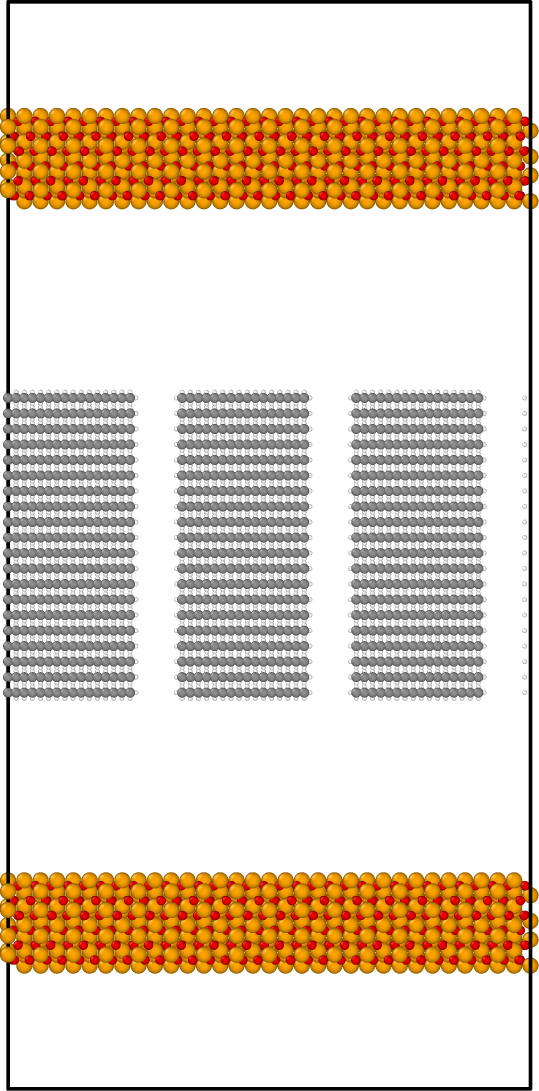
\includegraphics[width=0.150\textwidth]{Data/Images/1_initial.png}};
    			\support{3}{{(\textwidth-\textwidth/10)*0.00+\textwidth/20+\textwidth/24},					\textwidth/31};
    			\support{3}{{(\textwidth-\textwidth/10)*0.00+\textwidth/20+\textwidth/24+0.0669*\textwidth},	\textwidth/31};
    			\support{3}{{(\textwidth-\textwidth/10)*0.00+\textwidth/20+\textwidth/24},					0.278\textwidth}[180];
    			\support{3}{{(\textwidth-\textwidth/10)*0.00+\textwidth/20+\textwidth/24+0.0669*\textwidth},	0.278\textwidth}[180];
			%%%%%
			\node[anchor=south west,inner sep=0] (fig_Steps1) at ({(\textwidth-\textwidth/10)*0.25+\textwidth/20},0){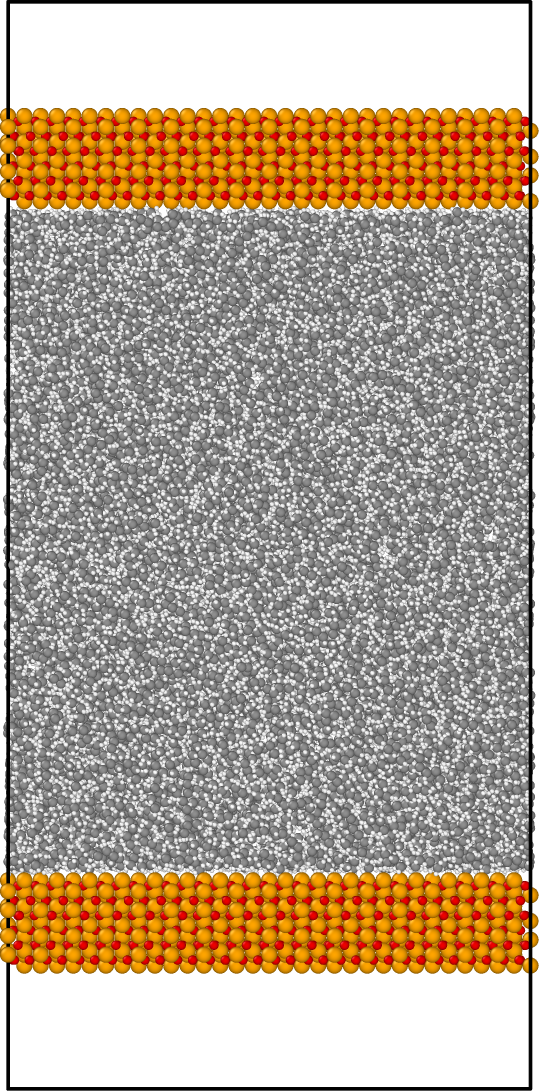
\includegraphics[width=0.150\textwidth]{Data/Images/2_equilibration.png}};
    			\support{3}{{(\textwidth-\textwidth/10)*0.25+\textwidth/20+\textwidth/24},					\textwidth/31};
    			\support{3}{{(\textwidth-\textwidth/10)*0.25+\textwidth/20+\textwidth/24+0.0669*\textwidth},	\textwidth/31};
    			\support{3}{{(\textwidth-\textwidth/10)*0.25+\textwidth/20+\textwidth/24},					0.278\textwidth}[180];
    			\support{3}{{(\textwidth-\textwidth/10)*0.25+\textwidth/20+\textwidth/24+0.0669*\textwidth},	0.278\textwidth}[180];
			%%%%%
			\node[anchor=south west,inner sep=0] (fig_Steps2) at ({(\textwidth-\textwidth/10)*0.50+\textwidth/20},0){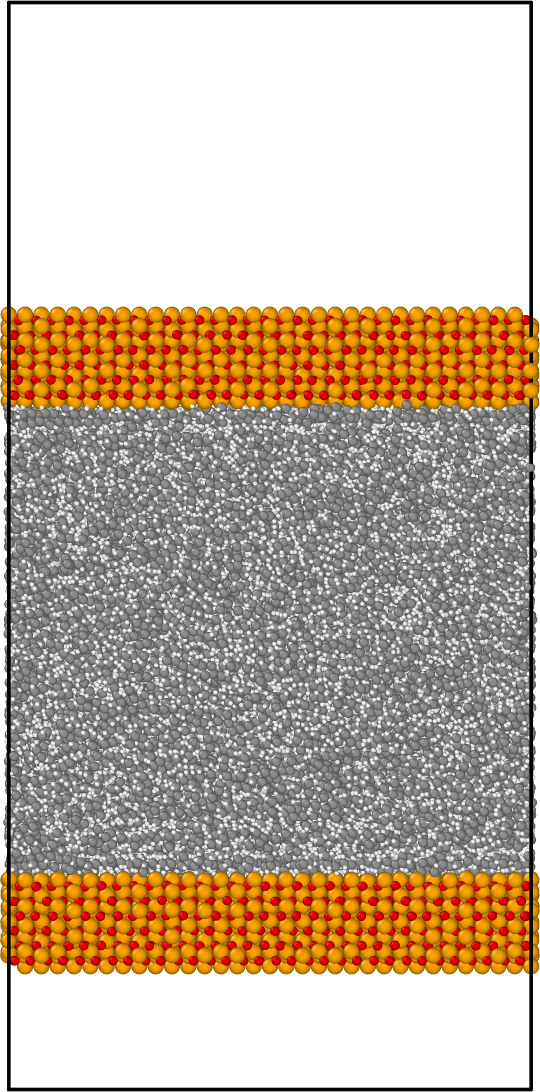
\includegraphics[width=0.150\textwidth]{Data/Images/3_Compression.png}};
    			\support{3}{{(\textwidth-\textwidth/10)*0.50+\textwidth/20+\textwidth/24},						\textwidth/31};
    			\support{3}{{(\textwidth-\textwidth/10)*0.50+\textwidth/20+\textwidth/24+0.0669*\textwidth},		\textwidth/31};
			\lineload{1}	{{(\textwidth-\textwidth/10)*0.50+\textwidth/20+\textwidth/110},					0.21*\textwidth}
						{{(\textwidth-\textwidth/10)*0.50+\textwidth/20+\textwidth/110+0.0669*2*\textwidth},	0.21*\textwidth}[0.5][0.5][0.11];
			\notation{5}{{(\textwidth-\textwidth/10)*0.50+\textwidth/20+\textwidth/110},					0.21*\textwidth}
						{{(\textwidth-\textwidth/10)*0.50+\textwidth/20+\textwidth/110+0.0669*2*\textwidth},	0.21*\textwidth}[$P$][][above left=0.077\linewidth];

			%%%%%
			\node[anchor=south west,inner sep=0] (fig_Steps3) at ({(\textwidth-\textwidth/10)*0.75+\textwidth/20},0){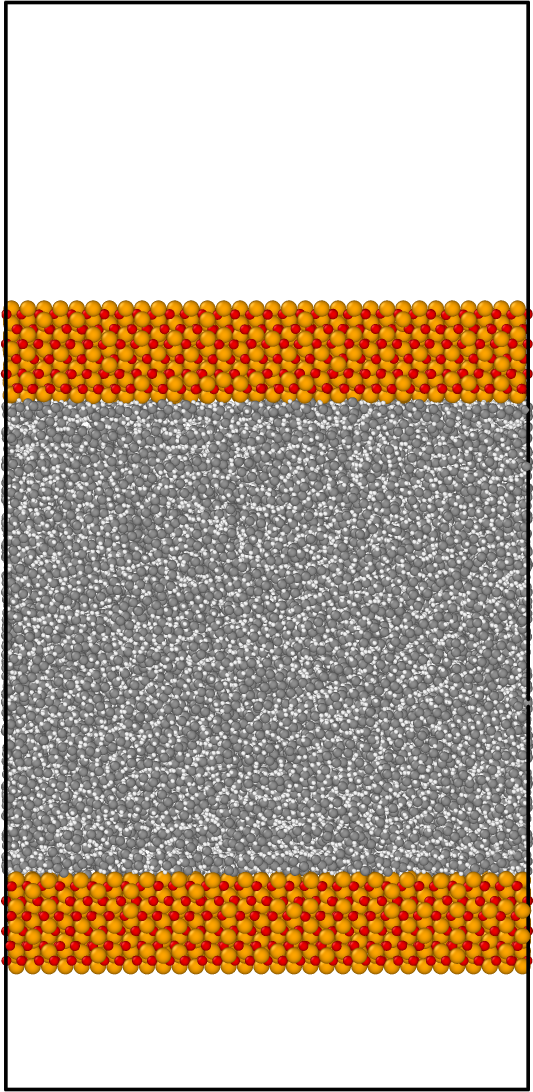
\includegraphics[width=0.148\textwidth]{Data/Images/4_shear.png}};
    			\support{4}{{(\textwidth-\textwidth/10)*0.75+\textwidth/20+\textwidth/24},						\textwidth/31};
    			\support{4}{{(\textwidth-\textwidth/10)*0.75+\textwidth/20+\textwidth/24+0.0669*\textwidth},		\textwidth/31};
			\lineload{1}	{{(\textwidth-\textwidth/10)*0.75+\textwidth/20+\textwidth/110},					0.21*\textwidth}
						{{(\textwidth-\textwidth/10)*0.75+\textwidth/20+\textwidth/110+0.0669*2*\textwidth},	0.21*\textwidth}[0.5][0.5][0.11];
			\notation{5}{{(\textwidth-\textwidth/10)*0.75+\textwidth/20+\textwidth/110},					0.21*\textwidth}
						{{(\textwidth-\textwidth/10)*0.75+\textwidth/20+\textwidth/110+0.0669*2*\textwidth},	0.21*\textwidth}[$P$][][above left=0.077\linewidth];
		
			\node (I) at (0.83*\textwidth, 0.206*\textwidth) {$\frac{v}{2}$} ;
			\node (J) at (0.78*\textwidth, 0.206*\textwidth) {} ;
			\draw [<- , line width=0.006*\textwidth] (I) -- (J);

			\node (K) at (0.78*\textwidth, 0.0455*\textwidth) {$\frac{v}{2}$} ;
			\node (L) at (0.83*\textwidth, 0.0455*\textwidth) {} ;
			\draw [<- , line width=0.006*\textwidth] (K) -- (L);
			

			\filldraw[fill=SERorange, draw=black] 	(0,4.5) circle (0.6125*3/4) node {Fe};
			\filldraw[fill=SERred, draw=black]  		(0,3.5) circle (0.365*3/4) node {O};
			\filldraw[fill=SERgray, draw=black]  		(0,2.5) circle (0.385*3/4) node {C};
			\filldraw[fill=SERwhite, draw=black]  	(0,1.5) circle (0.185) node {H};


			\begin{scope}[x={(fig_Steps0.south east)},y={(fig_Steps0.north west)}]
				\draw [](0.12\textwidth,-0.05) node[]{a)}	;
				\draw [](0.12\textwidth+0.225\textwidth,-0.05) node[]{b)}	;
				\draw [](0.12\textwidth+0.45\textwidth,-0.05) node[]{c)}	;
				\draw [](0.12\textwidth+0.675\textwidth,-0.05) node[]{d)}	;

			\end{scope}
		\end{tikzpicture}

		\caption{General steps carried out for the preparation and NEMD simulation of   each of the the systems considered in the present work. The orange atoms represent iron (Fe), the red ones oxygen (O), the gray ones carbon (C), and the white ones hydrogen (H). a) System generation. b) Equilibration. c) Compresion. d) Shear. }
		\label{fig:Steps}
	\end{center}
\end{figure*}

%%%%%%%%%%%%%%%%%%%%%%%%%%%%%%%%%%%%%%%%%%%%%%%%%

\subsubsection{Segmental Orientation}

Particle models like MD allow to measure orientation of polymer segments explicitly by taking the orientation of a bond as a segment orientation. The segmental orientation \cite{Monnerie1983,Erman1985,Besbes1992} of the fluid in terms of the second Legendre polynomial $\left(P_2\right)$ is defined as:

\begin{equation}\label{eq:P_2}
\left\langle P_2 \right\rangle =\frac{3\left\langle \cos ^2 \alpha \right\rangle - 1}{2},
\end{equation}

where $\alpha$ is the angle between a chain segment and a reference axis. In practice, $\left\langle \cos ^2 \alpha \right\rangle$ is calculated in the following way:

\begin{equation}
\left\langle \cos ^2 \alpha \right\rangle = \frac{1}{N_\text{bonds}} \sum_{b=1}^{N_\text{bonds}} \left(\frac{\textbf{r}^b_{ij}}{r^b_{ij}} \cdot \mathbf{\hat \imath} \right)^2
\end{equation}

 in which $N_\text{bonds}$ is the total number of bonds, $\textbf{r}^b_{ij}$ is the difference between the positions of the two beads that form the bond $b$, and $\mathbf{\hat \imath}$ is the direction of the main axis. 
 
 In this work we are interested in  the changes of the orientation in the shearing direction, so we will only focus on  the segmental orientation with respect to $x$ projected in the $xz$ plane: $P_{2}^{xz}$. Note that, by definition,  if all the chains are parallel to the shearing direction $\langle P_{2}^{xz}\rangle=1 $; if all the chains are perpendicular to the surfaces   $\langle P_{2}^{xz} \rangle=-0.5$, and, interestingly, if all the chains are oriented at  \SI{45}{\degree} or if they are randomly oriented $\langle P_{2}^{xz}\rangle=0.25 $
 
%%%%%%%%%%%%%%%%%%%%%%%%%%%%%%%%%%%%%%%%%%%%%%%%%

\subsubsection{Mean squared end-to-end distance}


The  squared end-to-end distance  of a single polymer chain is defined as the square  of the magnitude of  the vector that points from one end of a polymer to the other end. for a system containing several polymer chains, the mean squared end-to-end distance $\left(\left< R^2 \right>\right)$ is given by the following equation \cite{Brown1994}:

\begin{equation}
	\left< R^2 \right> = \left<\left( \mathbf{r}_1 - \mathbf{r}_N \right)^2\right>
	\label{eq:e2e2}
\end{equation}

where, for each polymer chain,  $N$ is the number of atoms and  $ \mathbf{r}_i$ is the position vector of atom $i$. 

%%%%%%%%%%%%%%%%%%%%%%%%%%%%%%%%%%%%%%%%%%%%%%%%%

\subsubsection{Mean squared radius of gyration}

The mean squared radius of gyration $\left(\left< S^2 \right>\right)$  is the average squared distance of each atom in the polymer chain  from its centre of mass, as defined in the following equation\cite{Brown1994}:

\begin{equation}
	\left< S^2 \right> = \frac{\left< \sum_{i=1}^{N}  \left ( \lVert \mathbf{r}_i - \mathbf{r}_{\text{com}} \rVert \right)^2 \right>}{N}
\end{equation}

where, for each polymer chain,  $N$ is the number of atoms, $ \mathbf{r}_i$ is the position vector of atom $i$  and $\mathbf{r}_{\text{com}}$ is the centre of mass. 

%%%%%%%%%%%%%%%%%%%%%%%%%%%%%%%%%%%%%%%%%%%%%%%%%

\subsubsection{Mean squared displacement}

The mean squared displacement (MSD) of an atom  is a measure of the deviation between its  current  and its initial position. For a material block consisting of several atoms, the  MSD averaged over the number of atoms  $\left(N\right)$ can be used to quantify  diffusion. The MSD is defined as:

\begin{equation}
	\text{MSD} = \frac{1}{N}\sum_{i=1}^{N} \left( \mathbf{r}_i\left(t\right)-\mathbf{r}_i\left(0\right)\right)^2
\end{equation}

where   $\mathbf{r}_i\left(t\right)$ is a vector containing the coordinates of atom $i$ at time $t$.


%%%%%%%%%%%%%%%%%%%%%%%%%%%%%%%%%%%%%%%%%%%%%%%%%

\subsubsection{Temperature}

The temperature of the lubricant is calculated as classically done in molecular dynamics via the kinetic energy of the atoms but excluding the velocity component in the direction of the movement of the surfaces (x) to avoid contributions that are not related to the thermal vibration of the atoms. The measurements are averaged every 100 steps to damp the fluctuations that are  characteristic of such small systems.

%%%%%%%%%%%%%%%%%%%%%%%%%%%%%%%%%%%%%%%%%%%%%%%%%
%%%%%%%%%%%%%%%%%%%%%%%%%%%%%%%%%%%%%%%%%%%%%%%%%
%%%%%%%%%%%%%%%%%%%%%%%%%%%%%%%%%%%%%%%%%%%%%%%%%
\section{Equilibration}
\label{sec:eq}


The first thing that needs to be done when simulating long chains of polymers is to generate a fully equilibrated system. In the present work, a simple 'brute force' scheme is used. In this procedure, an initially (artificially) ordered set of chains is heated-up to  a certain temperature, and is left to evolve until equilibrium is reached. Although it is not particularly efficient,  thanks to its simplicity and to the fact that the present system sizes are not prohibitively large, a method of this type was selected to equilibrate the systems. 

Here we split the equilibration procedure in two steps. First, the systems are heated-up to \SI{2000}{\kelvin}  --using a Langevin thermostat on the fluid-- to accelerate the diffusion of the chains, and maintained at this temperature for \SI{10}{\nano\second}.  Then the systems are cooled down and re-equilibrated at  \SI{353}{\kelvin}, which is the initial temperature of the NEMD simulations presented in the following sections. This second step also lasts  \SI{10}{\nano\second}.

Three different criteria are considered to ensure that the systems have reached equilibrium. The first two, consist on verifying that there is convergence of the mean squared end-to-end distance $\left(\left< R^2 \right> \right)$ and of  the mean squared radius of gyration $\left(\left< S^2 \right> \right)$.

The evolution of $\left< R^2 \right>$ and   $\left< S^2 \right>$  for C16, C30 and C60 at \SI{2000}{\kelvin}   are presented on the main part of  Figures  \ref{fig:e2e2} and \ref{fig:rg2}. For the case of the longest chains, which are the ones with lower diffusivity,  these two quantities converge after approx. \SI{2e5}{} steps (\SI{0.2}{\nano\second}). The insets of the figures show the evolution of the same quantities but after reducing the temperature to    \SI{353}{\kelvin}; we notice that after \SI{1e7}{} steps (\SI{10}{\nano\second}), both $\left(\left< R^2 \right> \right)$ and   $\left(\left< S^2 \right> \right)$ have reached their equilibrium values for the three  chain lengths considered.


%\begin{gnuplot}[terminal=pdf]
%\end{gnuplot}

\pgfmathsetmacro{\SERFigwidth}{.035\linewidth}
\pgfmathsetmacro{\SERFigheight}{.026\linewidth}
\begin{figure}
    	\begin{center}
		\begin{gnuplot}[terminal=pdf, terminaloptions={size \SERFigwidth cm, \SERFigheight cm color solid}]
			set multiplot
			#set format x  '$10^{%L}$' 
			set format y  '$10^{%L}$' 
			#set format x  '%3.1e' 
			#set format y  '%3.1e' 
			set key top left
			set xlabel "Time [\\SI{}{\\nano\\second}]"  
			set ylabel "$\\left< R^2 \\right>  [\\SI{}{\\square\\angstrom}]$"
			set logscale x
			set logscale y
			set key noautotitle
			  plot  [1e-2:1e1] [:1e5]	'Data/Equilibration/C16/e2e2.plot' u ($1/1e6):($2) title 'C16' ,\
						'Data/Equilibration/C30/e2e2.plot' u ($1/1e6):($2)  title 'C30' ,\
						'Data/Equilibration/C60/e2e2.plot' u ($1/1e6):($2)  title 'C60'

			set origin 0.4,0.55
			set size 0.54,0.4
			unset xlabel
			unset ylabel
			set xtics(10, 15, 20)
			#set xtics ('$10^1$' 1e1,  '$1.5\mkern-5mu\times\mkern-5mu 10^1$' 1.5e1, '$2\mkern-5mu\times\mkern-5mu 10^1$' 2e1)
			set ytics font ',80'
			plot [1e1:2e1][]	'Data/Equilibration/C16/e2e2.plot' u ($1/1e6):($2) ,\
							'Data/Equilibration/C30/e2e2.plot' u ($1/1e6):($2) ,\
							'Data/Equilibration/C60/e2e2.plot' u ($1/1e6):($2) 
			unset multiplot
		\end{gnuplot}
		\caption{Evolution of the mean squared end-to-end distance $\left(\left< R^2 \right>\right)$ during the equilibration stage for the three considered alkane lengths: C16, C30 and C60. The main plot shows the initial equilibration at  \SI{2000}{\kelvin}; the inset the continuation at  \SI{353}{\kelvin}. Note that $1 \times 10^{6}$ steps correspond to  \SI{1}{\nano\second}.}
		\label{fig:e2e2}
	\end{center}
 \end{figure}


\pgfmathsetmacro{\SERFigwidth}{.035\linewidth}
\pgfmathsetmacro{\SERFigheight}{.026\linewidth}
\begin{figure}
    	\begin{center}
		\begin{gnuplot}[terminal=pdf, terminaloptions={size \SERFigwidth cm, \SERFigheight cm color solid}]
			set multiplot
			#set format x  '$10^{%L}$' 
			set format y  '$10^{%L}$' 
			set key top left
			set xlabel "Time [\\SI{}{\\nano\\second}]"  
			set ylabel "$\\left< S^2 \\right>  [\\SI{}{\\square\\angstrom}]$"
			set logscale x
			set logscale y
			set key noautotitle
			plot   [1e-2:1e1] [:1e4]	'Data/Equilibration/C16/Rg2.plot'  u ($1/1e6):($2) title 'C16' ,\
						'Data/Equilibration/C30/Rg2.plot'  u ($1/1e6):($2) title 'C30' ,\
						'Data/Equilibration/C60/Rg2.plot'  u ($1/1e6):($2) title 'C60'
			set origin 0.4,0.55
			set size 0.54,0.4
			unset xlabel
			unset ylabel
			set xtics(10, 15, 20)
			#set xtics ('$10^7$' 1e7,  '$1.5\mkern-5mu\times\mkern-5mu 10^7$' 1.5e7, '$2\mkern-5mu\times\mkern-5mu 10^7$' 2e7)
			set ytics font ',80'
			plot [1e1:2e1][]	'Data/Equilibration/C16/Rg2.plot' u ($1/1e6):($2) ,\
							'Data/Equilibration/C30/Rg2.plot' u ($1/1e6):($2) ,\
							'Data/Equilibration/C60/Rg2.plot' u ($1/1e6):($2) 
			unset multiplot
		\end{gnuplot}
		\caption{Evolution of the mean squared radius of gyration $\left(\left< S^2 \right>\right)$  during the equilibration stage for the three considered alkane lengths: C16, C30 and C60. The main plot shows the initial equilibration at  \SI{2000}{\kelvin}; the inset the continuation at  \SI{353}{\kelvin}. Note that $1 \times 10^{6}$ steps correspond to  \SI{1}{\nano\second}.}
		\label{fig:rg2}
	\end{center}
 \end{figure}


The last criterion, is based on the fact that a  polymer melt that is not properly equilibrated can present deformation on short length scales, and this deformation  is only relaxed after the chains have moved --at least-- their own size\cite{Auhl2003}.  In order to verify it, the mean squared displacement per atom $\left(\text{MSD}_{\text{atom}}\right)$ and per centre of mass of polymer chain $\left(\text{MSD}_{\text{CG}}\right)$ are followed during equilibration. 


Figure \ref{fig:msd} shows the  $\text{MSD}_{\text{atom}}$ and $\text{MSD}_{\text{CG}}$ for the three different systems. Just like in the two previous figures, the main plot is dedicated to the evolution at  \SI{2000}{\kelvin}. Note that due to the artificial way that the chains are first introduced into the system (see Figure \ref{fig:Steps}), the diffusivity of the longer chains is initially higher than that of the shorter chains.  If we take the length of a C60 chain to be approx. \SI{74}{\angstrom} (the angle between the C-C bonds is \SI{109.5}{\degree} and the C-C distance equal to \SI{1.54}{\angstrom}),  it can be seen that the chains move their own size after approx. \SI{3e6}{} to  \SI{4e6}{} steps (\SI{3}{\nano\second} to \SI{4}{\nano\second}). Taking a conservative approach, the systems are equilibrated during  \SI{1e7}{} steps (\SI{10}{\nano\second}). The insets show the evolution after the temperature has been decreased; here, as expected, the slope of the $\text{MSD}_{\text{atom}}$ and $\text{MSD}_{\text{CG}}$ curves is less steep than at higher temperatures. We take these last configurations as the fully equilibrated systems for the following NEMD simulations.


\pgfmathsetmacro{\SERFigwidth}{.035\linewidth}
\pgfmathsetmacro{\SERFigheight}{.026\linewidth}
\begin{figure}
    	\begin{center}
		\begin{gnuplot}[terminal=pdf, terminaloptions={size \SERFigwidth cm, \SERFigheight cm color solid}]
			set multiplot
			#set format x  '$10^{%L}$' #'10^{%L}'
			set format y  '$10^{%L}$' #'10^{%L}'
			set xlabel "Time [\\SI{}{\\nano\\second}]"  
			set ylabel "$\\text{MSD}  [\\SI{}{\\square\\angstrom}]$"
			set key at 1.0e1, 1e3
			set logscale x
			set logscale y
			set key noautotitle
			plot [1e-2:1e1][1e2:] 	'Data/Equilibration/C16/msd.plot' 	 u ($1/1e6):($2) lc 1 pt 4 title 'C16',\
			   			'Data/Equilibration/C30/msd.plot' 			 u ($1/1e6):($2) lc 2 pt 4 title 'C30',\
			   			'Data/Equilibration/C60/msd.plot' 			 u ($1/1e6):($2) lc 3 pt 4 title 'C60'
			set origin 0,0
			set size 1,1

			set key at 1.5e1, 1e3
			plot [1e-2:1e1][1e2:]	'Data/Equilibration/C16/msd_cg.plot'  u ($1/1e6):($2)  lc 1 pt 7 title '  ',\
			   			'Data/Equilibration/C30/msd_cg.plot' 		  u ($1/1e6):($2)  lc 2 pt 7 title '  ',\
			   			'Data/Equilibration/C60/msd_cg.plot' 		  u ($1/1e6):($2)  lc 3 pt 7 title '  '

			set origin 0.145,0.55
			set size 0.54,0.4
			unset xlabel
			unset ylabel
			set xtics(10, 15, 20)
			#set xtics ('$10^7$' 1e7,  '$1.5\mkern-5mu\times\mkern-5mu 10^7$' 1.5e7, '$2\mkern-5mu\times\mkern-5mu 10^7$' 2e7)
			set ytics font ',80'
			plot [1e1:2e1][]	'Data/Equilibration/C16/msd.plot'  u ($1/1e6):($2) every 50 lc 1 pt 4 ,\
							'Data/Equilibration/C30/msd.plot'  u ($1/1e6):($2) every 50  lc 2 pt 4,\
							'Data/Equilibration/C60/msd.plot'  u ($1/1e6):($2) every 50  lc 3 pt 4,\
							'Data/Equilibration/C16/msd_cg.plot'  u ($1/1e6):($2) every 50  lc 1 pt 7,\
							'Data/Equilibration/C30/msd_cg.plot'  u ($1/1e6):($2) every 50  lc 2 pt 7,\
							'Data/Equilibration/C60/msd_cg.plot'  u ($1/1e6):($2) every 50  lc 3 pt 7


			unset multiplot
		\end{gnuplot}
		\caption{Evolution of the mean squared displacement (MSD)  during the equilibration stage for the three considered alkane lengths: C16, C30 and C60. The main plot shows the initial equilibration at  \SI{2000}{\kelvin}; the inset the continuation at  \SI{353}{\kelvin}. The full circles represent the mean squared displacement per atom $\left(\text{MSD}_{\text{atom}}\right)$ while the empty squares the mean squared displacement per centre of mass of polymer chain $\left(\text{MSD}_{\text{CG}}\right)$. Note that $1 \times 10^{6}$ steps correspond to  \SI{1}{\nano\second}.}
		\label{fig:msd}
	\end{center}
 \end{figure}


%%%%%%%%%%%%%%%%%%%%%%%%%%%%%%%%%%%%%%%%%%%%%%%%%
%%%%%%%%%%%%%%%%%%%%%%%%%%%%%%%%%%%%%%%%%%%%%%%%%
%%%%%%%%%%%%%%%%%%%%%%%%%%%%%%%%%%%%%%%%%%%%%%%%%
\section{Compression}

After the systems are fully equilibrated, a uniform pressure perpendicular to the surface is applied by blocking all the frozen atoms in the bottom wall, and applying a downwards force along the $z$ axis on the frozen Fe atoms in the top wall (see figures \ref{fig:Regions} and \ref{fig:Steps}c). The force is only applied on the Fe atoms --and not on the O-- due to the difference in their mass: if a force of the same magnitude  were applied to both species, different accelerations would be obtained and the structure of the walls could change. Three different pressure  values are considered, namely \SI{0.5}{\giga\pascal}, \SI{1.0}{\giga\pascal} and \SI{1.5}{\giga\pascal}. 

\begin{figure}
    	\begin{center}
		\begin{tikzpicture}
			\node[anchor=south west,inner sep=0] (fig_regions) at (0,0){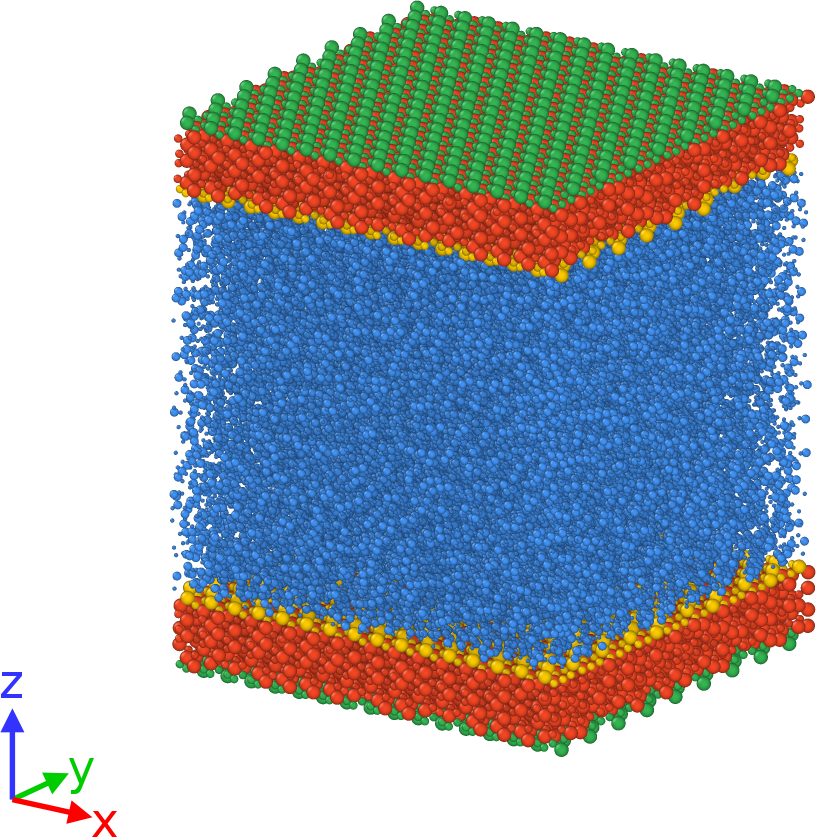
\includegraphics[width=0.25\textwidth]{Data/Images/5_region.png}};
			\begin{scope}[x={(fig_regions.south east)},y={(fig_regions.north west)}]
				\draw [](0,0.8) node[text width=1cm,align=center]{Top\\Wall}	;
				\draw [](0,0.53) node[]{Fluid}	;
				\draw [](0,0.27) node[text width=1cm,align=center]{Bottom\\Wall}	;

				\draw [decorate,decoration={brace}] (0.17,0.76) -- (0.17,0.86);
				\draw [decorate,decoration={brace}] (0.17,0.295) -- (0.17,0.755);
				\draw [decorate,decoration={brace}] (0.17,0.19) -- (0.17,0.29);

				\node (A) at (0.6,0.9) {} ;
				\node (B) at (1.0,1.0) [SERgreen]{Frozen} ;
				\draw [SERgreen, <- , line width=0.006*\textwidth] (A) -- (B);

				\node (C) at (0.8,0.78) {} ;
				\node (D) at (1.2,0.9) [SERorange2] {Thermostat} ;
				\draw [SERorange2, <- , line width=0.006*\textwidth] (C) -- (D);

				\node (E) at (0.8,0.74) {} ;
				\node (F) at (1.2,0.7) [SERyellow]{Free} ;
				\draw [SERyellow, <- , line width=0.006*\textwidth] (E) -- (F);
			\end{scope}
		\end{tikzpicture}
		\caption{Structure and regions of a typical system for the simulation of confined lubricants. The system is divided in three regions, namely, the fluid, and the top and bottom walls. Within each wall, the \textit{frozen} atoms (green) are used to apply the shearing and compressive constraints, and  the \textit{thermostat} atoms (orange) to control the temperature. Both the \textit{free} (yellow) and fluid (blue) atoms are left unconstrained.}
		\label{fig:Regions}
	\end{center}
\end{figure}


For the compression (and shearing) stages, the Langevin thermostat applied on the fluid during the equilibration stage is deactivated to avoid affecting dynamics of the lubricant;  the temperature of the system is then controlled only by a Langevin thermostat applied on the  \textit{thermostat} atoms on the surfaces (see Figure \ref{fig:Regions}). The thermostat  was applied exclusively in the direction perpendicular to both the sliding and compression (y). Note that the thermostat is not applied to the layer of atoms in contact with the lubricant.

The compression phase is performed in two steps: first, the pressure  is linearly incremented during  \SI{1e7}{} steps (\SI{10}{\nano\second}); and, second,  the pressure is maintained for the same amount of time. During this phase, we monitor the density of  the fluid region and the  pressure  on the bottom wall to  ensure that the system reaches equilibrium. In the case of the pressure, as expected, the measured values in all cases coincide with the desired applied pressures. For the densities,  we notice that the simulation time is long enough to obtain a stable value; the different final densities are presented in Table \ref{tab:rho}. These values  correspond to the average density of the last  \SI{1e6}{} steps (\SI{1}{\nano\second})  of the compression phase. Consistent with experimental results available in the literature\cite{Griesbaum2000}, we see an increase in density with the length of the chains and with the pressure.


\begin{table}
	\caption{Measured density values for confined alkanes  with three different chain lengths (C16, C30 and C60) at three different pressures (\SI{0.5}{\giga\pascal}, \SI{1.0}{\giga\pascal} and \SI{1.5}{\giga\pascal}).}   
	\centering     
	\begin{tabular}{c | l l  l}
		\hline\hline\\ [-2ex]

		
										&	\multicolumn{3}{c}{ $\rho \, [\SI{}{\kilogram\per\cubic\meter}]$} \\

		\hline\\ [-2ex]
		\backslashbox{Chain \\ Length}{P $[\SI{}{\giga\pascal}]$}	&	0.5		&	1.0		&	1.5	\\

		\hline\\ [-2ex]
		16C								&	0.87	&	0.93	&	0.98	\\
		30C								&	0.90	&	0.96	&	1.00	\\	
		60C								&	0.91	&	0.97	&	1.01	\\	

		\hline\hline    \\[-2ex]
	\end{tabular}
	\label{tab:rho}  
\end{table}


Equilibrium is reached via the movement and reorganisation in layers  of the polymer chains: the closer the chains are to the walls, the better defined is this layered structure. The polymer chains that are farther away  from the walls tend not to be so well organised and, for higher pressures and longer chain lengths, an amorphous-like region is formed. The formation of the amorphous regions is due to the fact that it is more difficult for longer chains to diffuse and find a more ordered and energetically favourable configuration, especially at higher pressures; this results, concurrently,  in  higher densities for longer chains (see Table \ref{tab:rho}). Note that this is in contrast with the behaviour of atomic fluids, which have the tendency to form ordered structures when subjected to higher pressures. 



%%%%%%%%%%%%%%%%%%%%%%%%%%%%%%%%%%%%%%%%%%%%%%%%%
%%%%%%%%%%%%%%%%%%%%%%%%%%%%%%%%%%%%%%%%%%%%%%%%%
%%%%%%%%%%%%%%%%%%%%%%%%%%%%%%%%%%%%%%%%%%%%%%%%%
\section{Shear}

Once the polymer melts are fully equilibrated at the desired pressures (\SI{0.5}{\giga\pascal}, \SI{1.0}{\giga\pascal}, \SI{1.5}{\giga\pascal}) we proceed to study the response of the lubricant to a shear deformation at applied  at the surfaces. The shearing deformation is applied by rigidly displacing the frozen atoms of the $\text{Fe}_2\text{O}_3$ surfaces in opposite directions along the $x$ axis (see Figure \ref{fig:Steps}). We consider the following absolute shearing velocities: \SI{20}{\meter\per\second}, \SI{50}{\meter\per\second} and \SI{100}{\meter\per\second}.


%%%%%%%%%%%%%%%%%%%%%%%%%%%%%%%%%%%%%%%%%%%%%%%%%

\subsection{Transient State}

Similarly to what was done in Section \ref{sec:eq} to verify that equilibrium was reached, we measure the evolution of three quantities to ensure that the shear simulations reach a steady state, namely,  the squared end-to end distance $\left(\left< R^2 \right> \right)$, the segmental orientation $\left(\left<P_{2}^{xz} \right> \right)$ and the lateral (friction) force $\left(F_L \right)$ on the surfaces. In general, the transition from a well equilibrated polymer melt to a steady state behaviour in shear is very similar for all the considered pressures and chain lengths. In general, a steady state is reached faster for shorter chains, higher shearing velocities and lower pressures. As a representative case, we will focus on the chain length C30 at a pressure of  \SI{1.0}{\giga\pascal}.
 
The evolution of these three quantities for the chain length C30 at a pressure of  \SI{1.0}{\giga\pascal} and the three selected shearing velocities is presented in Figure \ref{fig:SS}.


\pgfmathsetmacro{\SERFigwidth}{.035\linewidth}
\pgfmathsetmacro{\SERFigheight}{.036\linewidth}
\begin{figure}
    	\begin{center}
		\begin{gnuplot}[terminal=pdf, terminaloptions={size \SERFigwidth cm, \SERFigheight cm color solid}]
			set multiplot layout 4,1 rowsfirst
			set format x ' '
			unset xlabel

			set key bottom right
			set key samplen  0.0
			set ylabel "$\\left< R^2\\right>  \\,[\\SI{}{\\square\\angstrom}]$"          
			set label at graph 0.03,0.89 left "a)"
			set lmargin at screen 0.25; set rmargin at screen 0.9
			set tmargin at screen 1.00; set bmargin at screen 0.775
			set ytics 280,40,400 
			plot [:1100][260:440] 	'Data/Shear/C30/1.0GPa/10m_s/e2e2.plot_s.plot'  u  (($1/1e6)*10):($2) lt 3 pt 3 notitle  , 'Data/Shear/C30/1.0GPa/10m_s2/e2e2.plot_s.plot'  u (($1/1e6)*10):($2)  lt 3 pt 3 notitle ,\
								'Data/Shear/C30/1.0GPa/20m_s/e2e2.plot_s.plot'  u  (($1/1e6)*20):($2) lt 4 pt 4 notitle  , 'Data/Shear/C30/1.0GPa/20m_s2/e2e2.plot_s.plot'  u (($1/1e6)*20):($2)  lt 4 pt 4 notitle ,\
								'Data/Shear/C30/1.0GPa/50m_s/e2e2.plot_s.plot'   u (($1/1e6)*50):($2) lt 5 pt 5 notitle  , 'Data/Shear/C30/1.0GPa/50m_s2/e2e2.plot_s.plot' u  (($1/1e6)*50):($2)  lt 5 pt 5 notitle ,\
								'Data/Shear/C30/1.0GPa/100m_s/e2e2.plot_s.plot' u  (($1/1e6)*100):($2) lt 10 pt 10 notitle  , 'Data/Shear/C30/1.0GPa/100m_s2/e2e2.plot_s.plot' u (($1/1e6)*100):($2) lt 10 pt 10  notitle 
			
			unset label
			set tmargin at screen 0.775; set bmargin at screen 0.550
			set ytics 0.3, 0.1, 0.5			
			set ylabel "$\\left<P_{2}^{xz}\\right>$"        
			set label at graph 0.03,0.89 left "b)"  
			plot  [:1100][0.25:0.6]	'Data/Shear/C30/1.0GPa/10m_s/P2XZ_s.plot' u   (($1/1e6)*10):($2) lt 3 pt 3 title '' , 'Data/Shear/C30/1.0GPa/10m_s2/P2XZ_s.plot' u   (($1/1e6)*10):($2) lt 3 pt 3 notitle  ,\
								'Data/Shear/C30/1.0GPa/20m_s/P2XZ_s.plot' u   (($1/1e6)*20):($2) lt 4 pt 4 title '' , 'Data/Shear/C30/1.0GPa/20m_s2/P2XZ_s.plot' u   (($1/1e6)*20):($2) lt 4 pt 4 notitle  ,\
								'Data/Shear/C30/1.0GPa/50m_s/P2XZ_s.plot' u  (($1/1e6)*50):($2)  lt 5 pt 5 title '' , 'Data/Shear/C30/1.0GPa/50m_s2/P2XZ_s.plot' u  (($1/1e6)*50):($2)  lt 5 pt 5 notitle ,\
								'Data/Shear/C30/1.0GPa/100m_s/P2XZ_s.plot' u  (($1/1e6)*100):($2) lt 10 pt 10 title '' , 'Data/Shear/C30/1.0GPa/100m_s2/P2XZ_s.plot' u (($1/1e6)*100):($2) lt 10 pt 10 notitle 

			unset label
			set tmargin at screen 0.550; set bmargin at screen 0.325
			set ytics 30, 30, 120 
			set ylabel "$F_L \\, [\\SI{}{\\mega\\pascal}]$"          
			set label at graph 0.03,0.89 left "c)"
			plot  [:1100][20:150]	'Data/Shear/C30/1.0GPa/10m_s/fc_ave.dump.plot' u (($1/1e6)*10):($2/10)  lt 3 pt 3 notitle  , 'Data/Shear/C30/1.0GPa/10m_s2/fc_ave.dump.plot' u (($1/1e6)*10):($2/10)   lt 3 pt 3 notitle   ,\
							'Data/Shear/C30/1.0GPa/20m_s/fc_ave.dump.plot' u (($1/1e6)*20):($2/10)  lt 4 pt 4 notitle  , 'Data/Shear/C30/1.0GPa/20m_s2/fc_ave.dump.plot' u (($1/1e6)*20):($2/10)   lt 4 pt 4 notitle   ,\
							'Data/Shear/C30/1.0GPa/50m_s/fc_ave.dump.plot' u (($1/1e6)*50):($2/10)   lt 5 pt 5 notitle  , 'Data/Shear/C30/1.0GPa/50m_s2/fc_ave.dump.plot'  u (($1/1e6)*50):($2/10)  lt 5 pt 5 notitle  ,\
							'Data/Shear/C30/1.0GPa/100m_s/fc_ave.dump.plot' u (($1/1e6)*100):($2/10) lt 10 pt 10 notitle  , 'Data/Shear/C30/1.0GPa/100m_s2/fc_ave.dump.plot'  u (($1/1e6)*100):($2/10) lt 10 pt 10 notitle  

			unset label
			set format x '%g'
			set xlabel "Distance [\\SI{}{\\nano\\meter}]"  
			set tmargin at screen 0.325; set bmargin at screen 0.10
			#set label at graph 1.01,0.1 left "$\\times 10^{6}$"
			set ytics 300,100,700
			set ylabel "$T \\, [\\SI{}{\\kelvin}]$"          
			set label at graph 0.03,0.89 left "d)"
			plot  [:1100][280:750] 	'<grep c_temp_fluid Data/Shear/C30/1.0GPa/10m_s/log.comp_shear.plot'     u (($0/1000)*10):($6)        lt 3    pt 3    notitle ,\
								'<grep temp_flu Data/Shear/C30/1.0GPa/10m_s2/log.comp_shear.plot'   u (($0/1000+20)*10):($6) lt 3    pt 3    title  "\\SI{10}{\\meter\\per\\second}" ,\
								'<grep c_temp_fluid Data/Shear/C30/1.0GPa/20m_s/log.comp_shear.plot'     u (($0/1000)*20):($6)        lt 4    pt 4    notitle ,\
								'<grep c_temp_fluid Data/Shear/C30/1.0GPa/20m_s2/log.comp_shear.plot'   u (($0/1000+10)*20):($6) lt 4    pt 4    title  "\\SI{20}{\\meter\\per\\second}" ,\
								'<grep c_temp_fluid Data/Shear/C30/1.0GPa/50m_s/log.comp_shear.plot'     u (($0/1000)*50):($6)        lt 5    pt 5    notitle ,\
								'<grep c_temp_fluid Data/Shear/C30/1.0GPa/50m_s2/log.comp_shear.plot'   u (($0/1000+5)*50):($6)   lt 5    pt 5     title  "\\SI{50}{\\meter\\per\\second}" ,\
								'<grep c_temp_fluid Data/Shear/C30/1.0GPa/100m_s/log.comp_shear.plot'   u (($0/1000)*100):($6)     lt 10  pt 10   notitle ,\
								'<grep c_temp_fluid Data/Shear/C30/1.0GPa/100m_s2/log.comp_shear.plot' u (($0/1000+5)*100):($6) lt 10  pt 10  title  "\\SI{100}{\\meter\\per\\second}"
			unset multiplot
		\end{gnuplot}

		\caption{Evolution of the a) mean squared end-to-end distance $\left(\left< R^2 \right>\right)$, b) the average segmental orientation  $\left(\left<P_{2}^{xz}\right>\right)$, c) the lateral (friction) force  $\left(F_L\right)$ and d) the temperature $\left(T\right)$ for a system with alkane chains of length C30 at a pressure of \SI{1.0}{\giga\pascal} and  three  shearing velocities. The transient state begins with the application of the shear displacement of the surfaces and ends when  steady state is attained. Note that $1 \times 10^{6}$ steps correspond to  \SI{1}{\nano\second}.}
		\label{fig:SS}
	\end{center}
 \end{figure}

%%%%%%%%%%%%%%%%%%%%%%%%%%%%%%%%%%%
\subsubsection{End-to-end distance}

Since the initial configuration is the same for all the shearing velocities  they all have an initial value of  $\left< R^2 \right> = \SI{282.8}{\angstrom\squared}$. Once the surfaces start to move, and the lubricant to be sheared, there is virtually no change in $\left< R^2 \right> $ for a short amount of time. The reason for this phenomenon is that the surfaces are set in motion  instantaneously, that is, the final velocity is reached in only one time step.  During this time, the lubricant has a solid like behaviour and slides with respect to one of the surfaces, as evidenced by a discontinuity in the velocity field (see Figure \ref{fig:VelProf_MDP}).    For the case C30, \SI{1.0}{\giga\pascal} and \SI{50}{\meter\per\second} this ``plug'' flow  behaviour  lasts for about \SI{1e6}{} steps  -- see Figure \ref{fig:SS}a for the evolution of $\left< R^2 \right> $ with time.

\pgfmathsetmacro{\SERFigwidth}{.035\linewidth}
\pgfmathsetmacro{\SERFigheight}{.026\linewidth}
\begin{figure}
    	\begin{center}
		\begin{gnuplot}[terminal=pdf, terminaloptions={size \SERFigwidth cm, \SERFigheight cm color solid}]
			set multiplot layout 2,1 rowsfirst
			set format x ' '
			unset xlabel

			set key bottom right
			set key samplen  0.0
			set label at graph 0.03,0.89 left "a)"
			set lmargin at screen 0.25; set rmargin at screen 0.9
			set tmargin at screen 1.00; set bmargin at screen 0.55
			set ylabel "x Velocity $\\left[ \\SI{}{\\meter\\per\\second} \\right]$"
			set key noautotitle
			set xrange [-50:50]
			set yrange [-30:30]
			set ytics -40,20,40
			plot  	'Data/Shear/C30/1.0GPa/50m_s/vel_prof_x_s_50.dump.plot' u ($2-37.01):($4*100) w l  lt 7 lw 2  ,\
					'Data/Shear/C30/1.0GPa/50m_s/vel_prof_x_s_200.dump.plot' u ($2-37.77):($4*100) w l  lt 8 lw 2  ,\
					'Data/Shear/C30/1.0GPa/50m_s/vel_prof_x_s_500.dump.plot' u ($2-37.52):($4*100) w l  lt 9 lw 2  
					
			unset label

			set format x '%g'

			set tmargin at screen 0.55; set bmargin at screen 0.10
			set label at graph 0.03,0.89 left "b)"
			set key top center
			set xlabel "z coordinate"  
			set ylabel "AMD $\\left[ \\SI{}{\\gram\\per\\cubic\\centi\\meter} \\right]$ "
			set ylabel offset -1,0
			set ytics 0,1,4
			set yrange [0:3]
			set key noautotitle
			plot  	'Data/Shear/C30/1.0GPa/50m_s/fluid_mdp_z_s_0.dump.plot' u ($2-35.77):($4) w l  lt 10 lw 2   title "Step $\\SI{0}{}$" ,\
				  	'Data/Shear/C30/1.0GPa/50m_s/fluid_mdp_z_s_50.dump.plot' u ($2-37.01):($4) w l  lt 7 lw 2   title "Step $\\SI{0.5e6}{}$" ,\
				  	'Data/Shear/C30/1.0GPa/50m_s/fluid_mdp_z_s_200.dump.plot' u ($2-37.77):($4) w l  lt 8 lw 2   title "Step $\\SI{2e6}{}$" ,\
				  	'Data/Shear/C30/1.0GPa/50m_s/fluid_mdp_z_s_500.dump.plot' u ($2-37.52):($4) w l  lt 9  lw 2  title "Step $\\SI{5e6}{}$" 
			unset multiplot
		\end{gnuplot}
		\caption{a) Velocity profiles along x at three different times during the transient state of the simulation. b) Atomic Mass Density profile (AMD) along z $\left(\rho \left(z\right) \right)$ at the beginning and  three other times during the transient state of the simulation. In both cases, Results are presented for the case of  C30,  \SI{1.0}{\giga\pascal} and  \SI{50}{\meter\per\second}.}
		\label{fig:VelProf_MDP}
	\end{center}
 \end{figure}


As shear continues to be applied to the system,  we see a linear increment of $\left< R^2 \right> $ until an equilibrium value is reached. For the case C30 and \SI{1.0}{\giga\pascal}  the steady state is reached after \SI{10e6}{}, \SI{4e6}{} and \SI{2e6}{} steps for the velocities  \SI{20}{\meter\per\second}, \SI{50}{\meter\per\second} and \SI{100}{\meter\per\second}, which suggests that the equilibration of  $\left< R^2 \right> $ is not time but shearing-distance dependent, as shown in Figure \ref{fig:SS}a and previously seen experimentally\cite{Drummond2000}.   A change in the structure of the polymer chains occurs while the simulation reaches steady state: initially the  chains are folded and, as the system is deformed, they unfold and stretch causing an increase in the value of  $\left< R^2 \right> $, until a steady state is attained. One of the reasons  for the increase  is that the chains that are closer to the surface are attracted by it while simultaneously being pulled by the flow. Note that lower shearing velocities result in more elongated chains.


%%%%%%%%%%%%%%%%%%%%%%%%%%%%%%%%%%%

\subsubsection{Segmental orientation}
 
 According to theory, and as mentioned previously, the equilibrium average segmental orientation of an ideal chain (or freely-jointed chain)  should be $\langle P_{2}^{xz}\rangle=0.25$. Nevertheless, in the cases considered in this work, the equilibrium value before any shearing deformation is higher. For instance, for the case C30 and  \SI{1.0}{\giga\pascal}, $\langle P_{2}^{xz}\rangle=0.32$ (see Figure \ref{fig:SS}b), indicating that there is  a defined preferential orientation caused by the presence of the surfaces; the surfaces  drive  the chains off the ideal orientation towards a more horizontal position (parallel to the surface). %, see Figure \ref{fig:steady}).   
 
The chains adjacent  to the surfaces tend to lie horizontally  to form a first  layer of lubricant. This first layer itself has an influence in the orientations of the neighbouring chains, producing  a cascading effect that results in the formation of  a layered structure, as show in figure \ref{fig:VelProf_MDP} where the mass density profile of the chains is presented for the case of  C30,  \SI{1.0}{\giga\pascal} and  \SI{50}{\meter\per\second} --for the information before shearing, refer to Step 0 in the figure. 





Although we also see a linear increase of $\left<P_{2}^{xz} \right> $ as shear is applied, the path towards a steady state of  $\left<P_{2}^{xz} \right> $ starts earlier than that of  $\left< R^2 \right> $. The chains begin to reorient themselves even during the ``plug'' flow regime. %This can be seen, for example, in Figure  \ref{fig:steady}b, where some of the chains in the bulk  are still folded but with an orientation close to the steady state value of  $\left<P_{2}^{xz}\right>=0.50$, which corresponds to an angle of \SI{35.3}{\degree} measured from the $x$ towards the $z$ axis. 

The time needed for $\left<P_{2}^{xz} \right>$ to reach a steady state  is similar to that needed for the equilibration of  $\left< R^2 \right> $ and follows the same trend: faster shearing velocities lead the system  to reach faster a steady state, as shown in  Figure \ref{fig:SS}b.


%%%%%%%%%%%%%%%%%%%%%%%%%%%%%%%%%%%

\subsubsection{Lateral (Friction) force}

The lateral (friction) force $F_L$ is calculated from the simulations as the average total force in the $x$ direction acting on the outermost layer of atoms (frozen atoms in Figure \ref{fig:Regions}) in each of the slabs divided by their area. The time needed for $F_L$  to reach a steady state is consistent with the time  needed for $\left< R^2 \right> $ and $\left<P_{2}^{xz} \right> $, revealing a dependency of $F_L$ on these two quantities: $F_L$ will only reach a steady state after the chains are steadily oriented and elongated.


%%%%%%%%%%%%%%%%%%%%%%%%%%%%%%%%%%%

\subsubsection{Temperature}

The evolution of the temperature follows the same trend as the other studied parameters: for the same system,  higher shearing velocities reach a steady state faster. We also notice that, even though the temperature at the thermostated atoms at the surfaces is maintained at  \SI{353}{\kelvin}, the larger amount of kinetic energy inserted to the system due to the higher velocities causes more energy dissipation in the fluid and leads to a more pronounced increase of the  temperature.
%xxxx what happens in a case where the lubricant is solid



%%%%%%%%%%%%%%%%%%%%%%%%%%%%%%%%%%%%%%%%%%%%%%%%%

\subsection{Steady state}

Once the simulations reach a steady state, they are left to run for  \SI{5}{\nano\second} to  \SI{10}{\nano\second}  while maintaining constant the shearing velocity and the applied pressure. During the last  \SI{2}{\nano\second} of the simulation, the values of the average squared end-to-end distance $\left(\left< R^2 \right> \right)$,   average segmental orientation $\left<P_{2}^{xz} \right> $, and lateral (friction) force $\left(F_L\right)$ are measured and averaged; the results and analysis of these measurements are presented in this section.   


%At 0.5GPa the velocity does not contribute much to the friction


%%%%%%%%%%%%%%%%%%%%%%%%%%%%%%%%%%%%%%%%%%%%%%%%%

\subsubsection{End-to-end distance}

As previously defined in equation \ref{eq:e2e2}, the values of  the end-to-end distance are chain length dependent. In order to be able to compare the variation of $\left< R^2 \right> $ between the different chain lengths considered, we calculate instead the average squared end-to-end distance per bond: $\left< R^2 \right>/\left(N_\text{bonds}\right)^2$. The results of such calculations as a function of the applied pressure and shearing velocity are presented in Figure   \ref{fig:e2e2_v}.


\pgfmathsetmacro{\SERFigwidth}{.035\linewidth}
\pgfmathsetmacro{\SERFigheight}{.026\linewidth}
\begin{figure}
    	\begin{center}
		\begin{gnuplot}[terminal=pdf, terminaloptions={size \SERFigwidth cm, \SERFigheight cm color solid}]
			set key above
			set xlabel  "x Velocity $\\left[ \\SI{}{\\meter\\per\\second} \\right]$"  
			set ylabel "$\\left< R^2 \\right>/\\left(N_\\text{bonds}\\right)^2$ [\\SI{}{\\square\\angstrom}]"
			set key noautotitle
			p [:110][]	'Data/Shear/Compiled_e2e2_v.plot8.plot' i 0 u ($3):($6/($1-1)**2):($7/($1-1)**2) w errorbars title "$\\SI{0.5}{\\giga\\pascal}$" lt 1 lc 0 ps 2,\
				'Data/Shear/Compiled_e2e2_v.plot8.plot' i 1 u ($3):($6/($1-1)**2):($7/($1-1)**2) w errorbars title  "$\\SI{1.0}{\\giga\\pascal}$" lt 2 lc 0 ps 2,\
				'Data/Shear/Compiled_e2e2_v.plot8.plot' i 1 u ($3):($6/($1-1)**2) w l notitle lt 2 lc 1  lw 2 ,\
				'Data/Shear/Compiled_e2e2_v.plot8.plot' i 2 u ($3):($6/($1-1)**2):($7/($1-1)**2) w errorbars title  "$\\SI{1.5}{\\giga\\pascal}$" lt 3 lc 0 ps 2,\
				'Data/Shear/Compiled_e2e2_v.plot8.plot' i 2 u ($3):($6/($1-1)**2) w l notitle lt 3 lc 1 lw 2 ,\
				'Data/Shear/Compiled_e2e2_v.plot8.plot' i 3 u ($3):($6/($1-1)**2):($7/($1-1)**2) w errorbars notitle lt 1 lc 0 ps 2 ,\
				'Data/Shear/Compiled_e2e2_v.plot8.plot' i 0 u ($3):($6/($1-1)**2) w l title "C16" lt 1 lc 1 lw 2 ,\
				'Data/Shear/Compiled_e2e2_v.plot8.plot' i 3 u ($3):($6/($1-1)**2) w l title "C30" lt 1 lc 2 lw 2 ,\				
				'Data/Shear/Compiled_e2e2_v.plot8.plot' i 4 u ($3):($6/($1-1)**2) w l notitle lt 2 lc 2 lw 2 ,\
				'Data/Shear/Compiled_e2e2_v.plot8.plot' i 4 u ($3):($6/($1-1)**2):($7/($1-1)**2) w errorbars notitle lt 2 lc 0 ps 2,\
				'Data/Shear/Compiled_e2e2_v.plot8.plot' i 5 u ($3):($6/($1-1)**2) w l notitle lt 3 lc 2 lw 2 ,\
				'Data/Shear/Compiled_e2e2_v.plot8.plot' i 5 u ($3):($6/($1-1)**2):($7/($1-1)**2) w errorbars notitle lt 3 lc 0 ps 2 ,\
				'Data/Shear/Compiled_e2e2_v.plot8.plot' i 6 u ($3):($6/($1-1)**2):($7/($1-1)**2) w errorbars notitle lt 1 lc 0 ps 2 ,\
				'Data/Shear/Compiled_e2e2_v.plot8.plot' i 6 u ($3):($6/($1-1)**2) w l title 'C60' lt 1 lc 3 lw 2 ,\				
				'Data/Shear/Compiled_e2e2_v.plot8.plot' i 7 u ($3):($6/($1-1)**2) w l notitle  lt 2 lc 3 lw 2 ,\
				'Data/Shear/Compiled_e2e2_v.plot8.plot' i 7 u ($3):($6/($1-1)**2):($7/($1-1)**2) w errorbars notitle  lt 2 lc 0 ps 2,\
				'Data/Shear/Compiled_e2e2_v.plot8.plot' i 8 u ($3):($6/($1-1)**2) w l notitle  lt 3 lc 3 lw 2 ,\
				'Data/Shear/Compiled_e2e2_v.plot8.plot' i 8 u ($3):($6/($1-1)**2):($7/($1-1)**2) w errorbars notitle  lt 3 lc 0 ps 2,\
		\end{gnuplot}
		\caption{Average squared end-to-end distance per bond as a function of the shearing velocity measured after reaching steady state.}
		\label{fig:e2e2_v}
	\end{center}
 \end{figure}



In terms of the shearing velocities, the behaviour of $\left< R^2 \right>/\left(N_\text{bonds}\right)^2$ follows the same trend for all the chain lengths and pressures: higher shearing velocities result in more compact (less elongated) molecules. This behaviour is explained by the two following arguments:

First,  when the movement of the surfaces is slower, the  polymer chains have more time to organise themselves in layers parallel to the surfaces, as evidenced in the mass density profiles plotted in Figure \ref{fig:VelProf_MDP2}, where the peaks are more pronounced for  a velocity of \SI{20}{\meter\per\second} than for \SI{100}{\meter\per\second}. Then, as the chains position themselves in layers, they are  elongated by the opposite relative movement of the surfaces, resulting in larger values of $\left< R^2 \right>/\left(N_\text{bonds}\right)^2$ for slower shearing velocities.







\end{document}

%git pull
%git add -A
%git commit
%git push origin master